\documentclass{ieeeaccess}
\usepackage{cite}
\usepackage{amsmath,amssymb,amsfonts}
\usepackage{algorithmic}
\usepackage{graphicx}
\usepackage{textcomp}

\def\BibTeX{{\rm B\kern-.05em{\sc i\kern-.025em b}\kern-.08em
    T\kern-.1667em\lower.7ex\hbox{E}\kern-.125emX}}
\begin{document}
\history{Date of publication xxxx 00, 0000, date of current version xxxx 00, 0000.}
\doi{10.1109/ACCESS.2017.DOI}

\title{Deep Q Learning for Self Adaptive Distributed Microservices Architecture}
\author{\uppercase{Basel Magableh}\authorrefmark{1}, 
\uppercase{Muder Almiani\authorrefmark{2}, and Luca Longo}\authorrefmark{3}}
\address[1]{Technological University, Dublin, Ireland (e-mail: basel.magableh@dit.ie)}
\address[2]{Al-Hussein Bin Tala University, Ma'an, Jordan (e-mail: malmiani@my.bridgeport.edu)}
\address[3]{Technological University, Dublin, Ireland (e-mail: luca.longo@dit.ie)}
\tfootnote{}

\markboth
{Magableh \headeretal: Deep Q Learning for Self Adaptive Microservices Architecture  }
{Magableh \headeretal: Deep Q Learning for Self Adaptive Microservices Architecture}

\corresp{Corresponding author: Magableh B.  (e-mail: basel.magableh@dit.ie).}

\begin{abstract}
One desired aspect of a self-healing Microservices architecture is the ability to continuously monitor the operational environment, detect and observe anomalous behaviour, and provide a reasonable policy for self-scaling, self-healing, and self-tuning the computational resources to adapt a sudden changes in its operational environment dynamically at rune-time. The behaviour of Microservices architecture is continuously changing overtime, which makes it a challenging task to use a statistical model to identify normal and abnormal behaviour of the running services. The performance of the cluster nodes could fluctuate around the demand to accommodate scalability, orchestration and load balancing demands. To achieve highly level of self adaptability, this research implements Microservices architectures a MAPE-K model that employ Markov Decision Process (MDP) in identifying the transition model from one cluster state to another. Also, it employees a Deep Q-learning network (DQN) for dynamically selecting the adaptation action that fits in the current architecture state. Also this paper evaluates the effectiveness of using DQN and MDP agent to achieve high level of self-adaptability of Microservices architecture. We argue in this paper that such integration between DQN and MDP in MAPE-K model offers Microservices architecture with self-adaptability against the contextual changes in the operational environment. The self-adaptation property is achieved by means of parameter tuning and dynamic adjustment of the architecture configuration. We believe integrating DQN in the dynamic decision-making process improves the effectiveness of the adaptation and reduces the adaptation risk including resources over-provisioning and thrashing. Also, it preserving the cluster state by preventing multiple adaptation to take place at the same time. It also guarantees that the executed adaptation action returns the highest reward and achieve the adaptation goals.

%At the same time, the use of reinforcement learning guarantees that the learned knowledge from each pair of action-state is learned by the Deep Q-learning, which will prevent the adaptation manager from executing adaptation action that would fail and return negative reward. In the following section, we will describe the experiment setup and the tools used to construct the Microservices architecture. Also, we will describe the  structure of the neural network used in this experiment. 

 %This requires a model that is able to detect anomalies in real-time and generate a high rate of accuracy in detecting any anomalies and a low rate of false alarms. At the same time, it requires dynamic policy configuration that can be used to adapt the recent changes in the operational environment. This paper focuses on proposing a self-healing Microservices architecture, that is able to continuously monitor the operational environment, detects and observes anomalous behaviour, and provides a reasonable adaptation policy using multidimensional utility-based model. We argue in this paper that such model could offer self-scaling of Microservices architecture and adapt the sudden changes in the operational environment. The self-healing property is achieved by means of parameter tuning and dynamic adjustment of the cluster configuration. We believe integrating utility theory in the dynamic decision-making process improves the effectiveness of the adaptation and reduces the adaptation risk including resources over-provisioning and thrashing. Also, it preserving the cluster state by preventing multiple adaptation to take place at the same time
\end{abstract}

\begin{keywords}
Anomaly detection, Micoroservices Architecture, Q Learning, Runtime configuration, Self Healing, Reinforcement learning, Policy Approximation 
\end{keywords}

\titlepgskip=-15pt

\maketitle

\section{Introduction}
\label{sec:introduction}
\PARstart{M}{icroservices} architecture could be defined in the context of a service-oriented architecture as a composition of tiny fine-grained distributed loosely coupled building blocks of software components \cite{stubbs2015distributed}. Microservices improve software modularity and make the application easy to develop and maintain. With the rapid development of cloud infrastructures and virtualisation techniques, a high demand for building Microservices architectures in a complete virtualised environment has emerged. This need was met by introducing containers engine like Docker \footnote{https://www.docker.com} as well as cluster management framework such as Docker swarm \footnote{https://docs.docker.com/engine/swarm/}.  
The performance of Microservices running in cluster mode could fluctuate around the demand to accommodate scalability, orchestration and load balancing offered by the cluster leader \cite{stubbs2015distributed}.  It is essential for Microservice architecture to be able to reason about its own state and its surrounding environment in a closed control loop and act dynamically at runtime to achieve high level of adaptability \cite{Cheng:2008p3708}.   
Such level of self-adaptation requires the Microservices architecture to be able to observe its current state and provide a suitable adaptation action so it can adjust itself to reason about various contextual changes.

Nowadays, Microservices architecture does not have components that can guarantee continuous monitoring and adaptation of the operational environment. Also Microservices architecture can not offer the architecture with dynamic capability to reason  about context changes at run-time. 

To achieve such a high level of adaptability, a Microservices cluster, for instance, should have a component for continuously monitoring the cluster and a component for adaptation that can implement a reasonable reaction/scaling policy to accommodate the changes in the operating environment. This presents a challenge to build a self-adapting microservices architecture that can dynamically adjust its own behaviour and heal itself against anomalous behaviour detected at real-time. 

The proposed model in this paper offers Microservices architecture a self-adaptation property by following MAPE-K (Monitor-Analyse-Plan-Execute over a shared Knowledge) model.
Our model provides a mechanism for continuous monitoring, context detecting of anomalous behaviour , dynamic decision making using reinforcement learning, enabling dynamic adaptation horizontally or vertically based on the demand and the changes of the operational environment, and runtime verification and validation of the fitness of proposed adaptation strategy. 

To achieve highly level of self adaptability, this research implements a MAPE-K model that employ Markov Decision Process in identifying the transition model from one cluster state to another.  Also, it employees a Deep Q-learning network (DQN) that able to select the optimal adaptation action that returns the highest reward gained from executing the adaptation actions. At the same time, the use of  Deep Q-learning guarantees that the knowledge from each pair of action-state is used in selecting future adaptation action to avoid adaptation failure and provide the maximum level of availability, reliability and scalability.  

This paper is structured as follows:  Section \ref{sec:modelling} presents a model that can continuously observe Microservice architectures with Self-healing capabilities. Adaptation planing and execution is discussed in Section \ref{sec:mapk}. 
Section \ref{sec:evaluation} proposes a strategy for analysing and evaluating the capability of the model  to detect anomalous behaviours and to trigger suitable adaptation actions. The implementation of this model is discussed in Section \ref{sec:setup}. Section \ref{sec:disc} is focused on results found followed a by a critical discussion of the effectiveness of this model. Section \ref{sec:related-work} provides an overview of self-healing architectures and surveys the approaches for  anomaly detection, and run-time configurations. Section \ref{sec:Conclusion} summarises this research, highlighting its contribution and setting future work.

%\section{Related work}
\label{sec:related-work}
\subsection{Self-adaptive Software}
Self-adaptive software is characterised by a number of properties best referred to as autonomic \cite{jelasityself}. These the `self-* properties' include Self-organisation, Self-healing, Self-optimisation and Self-protection  \cite{horn:2001p3735}. Self-healing architecture refers to  the capability of discovering, diagnosing and reacting to disruptions. It can also anticipate potential problems and, accordingly, take suitable actions to prevent a failure \cite{horn:2001p3735}. Self-healing aspects of Microservices architectures requires a decision-making strategy that can work in real-time. This is essential for Microservice to reason about its own state and its surrounding environment in a closed control loop model and act accordingly \cite{Cheng:2008p3708}.  
Typically, a self-adapting system follows MAPE-K model (Monitor-Analyse-Plan-Execute over a shared Knowledge). a self-healing system should implements MAPE-K model including: Gathering of data related to the surrounding context (Context Sensing); Context observation and detection; Dynamic decision making; Adaptation execution to achieve the adaptation objectives defined as QoS; Verification and validation of the applied adaptation actions in terms of its ability to meet the adaptation objectives and meet the desired QoS.
\subsection{Context Sensing}

 However, there is many approaches are used for achieving high level of self-adaptability though Context sensing involving context collection, observation and detection of contextual changes in the operational environment \cite{Strang:2004p3770}. Also, the ability of the system to dynamically adjust its behaviour can be achieved using parameter-tuning \cite{Cheng:2009p3902}, component-based composition \cite{MariusMikalsen:2005ur}, or Middleware-based  approaches \cite{CheungFooWo:2007p1692}. Another important aspect of self-adaptive system is related to its ability to validate and verify the adaptation action at runtime based on Game theory \cite{Wei:2016ge}, Utility theory as in \cite{Menasce:2007vq,KonstantinosKakousis:2008ub}, or Model driven approach as in \cite{Sama:2008p3765}.

Context information (1) refers to any information that is computationally accessible and upon which behavioural variations depend \cite{Hirschfeld:2008p1620}. Context observation and detection approaches (2) are used to detect abnormal behaviour within the microservices architecture at run-time. Related work in context modelling, context detection and engineering self-adaptive software system are discussed in \cite{Salehie:2009p3693,Cheng:2008p3708,RogeriodeLemos:2011tj,Strang:2004p3770}.  
In dynamic decision making and context reasoning (3), the architecture should be able to monitor and detect normal/abnormal behaviour by continuously monitoring the contextual information found in the Microservices cluster. 

\subsection{Adaptation Planing and Execution}
In Microservices cluster, the performance of the cluster nodes could fluctuate around the demand to accommodate scalability, orchestration and load balancing issued by cluster leader. This requires a model that is able to detect anomalies in real-time and generate a high rate of accuracy in detecting any anomalies and a low rate of false alarms. In addition, there will be a set of variations that can be used by the system to adapt the changes in its operational environment. This requires a dynamic decision making that can calculate the utility of all possible adaptation actions based on the architecture constraints (i.e. number of replicas, number of nodes, desired objectives, metrics thresholds), anomaly score of the detected conditions (CPU, Memory, DISK I/O, Network I/O), and the confidence and accuracy of the anomaly score of the detected abnormal behaviour, and the desired/predicted cluster state. Then, the adaptation manager will execute the adaptation action and verifies its successfulness over the cluster architecture. Also, the adaptation manager will be able to self-tune and self-adjust the architecture parameters to meet high/low demand for services. Finally, the architecture will preserve the cluster state through the adaptation cycle (monitoring, observing, detecting, reacting, and verifying). This research focuses on finding a method to continuously observe and monitor the swarm cluster and be able to detect anomalous behaviour with a high accuracy and generate a low rate of false alarms. Then provide the architecture with adaptation strategies with high utility to reason about the detected anomalies and be able to self-adjust the architecture parameters and verifies the adaptation actions at runtime without human intervention.


\subsection{Anomaly Detection}

There are two phases for detecting anomalies in a software system: a training phase which involves profiling the normal behaviour of the system; a second phase aimed at testing the learned profile of the system with new data and employing it to detect normal/abnormal behaviours \cite{Patcha:2007hja}. 

Three major techniques for anomaly detection have emerged from the literature: statistical anomaly detection, data-mining and machine-learning based techniques. 

Within the statistical methods, a system observes the activity of the system and generates profiles of  system metrics to represent its behaviour. The system profile includes performance measures of the system resources such as CPU and Memory. For each measure, a separate profile is stored. Then, the current readings of the system are profiled and compared against the memorised past profile to calculate an anomaly score. This score is calculated by comparing all measures within the profile against a threshold specified by the developer. Once the system detects that the current readings of the system  are higher than this threshold, then these will be automatically categorised as  intrusions thus triggering an alert \cite{kruegel2003anomaly}. 

Various statistical anomaly detection systems have been proposed and they have some advantages \cite{anderson1995next,roesch1999snort}. 
One of this is that they can detect an anomaly without prior knowledge of the system. This can mitigate the common problem of a cold start found in machine learning techniques. Additionally, statistical anomaly detection provides accurate notifications of malicious attacks that occurred over long periods of times and it performs better in detecting denial-of-service attacks \cite{Patcha:2007hja}. 
However, a disadvantage is that a skilled attacker might train a statistical anomaly detection system to accept the abnormal behaviour as normal. It is difficult to determine the thresholds that make a balance between the likelihood of a false negative (the system fails to identify an activity as an abnormal behaviour) and the likelihood of a false positive (false alarms). Statistical methods need an accurate  model with a precise distribution of all measures. In practice, the behaviour of virtual machines/computers cannot be entirely be modelled using solely statistical methods.

With regard to data-mining approaches, data-mining is about finding insights which are statistically reliable, unknown previously, and actionable from data \cite{phua2010comprehensive}. The dataset must be available, relevant, adequate, and clean. The data mining process involves discovering a novel, distinguished and useful data pattern in large datasets to extract hidden relationships and information about the data. In general, there are two issues involved in the use of data mining in an anomaly detection system. First, there is a lack of a large dataset to be used by the algorithm containing lots of information about the architecture. Second, few approaches were targeting the anomaly detection system in Microservices architecture \cite{phua2010comprehensive}. Data mining based anomaly detection systems have three major difficulties which prevent them from being widely adopted in Microservices architecture \cite{Patcha:2007hja}. Firstly, the low accuracy of detecting anomalous behaviour \cite{gupta2016network,Patcha:2007hja}, as the data mining process would require large dataset with longer time interval to be able to improve the accuracy of detection. Most data mining techniques are heavily on computational resources, this negatively influences their adoption in a Microservices architecture \cite{Patcha:2007hja}. Additionally, usually a data mining method used to classify an attack within a specific system cannot be successfully employed within another system for the same purpose. This because the process of training, testing the model and performing classification of anomalies needs to be repeated with different data or architecture \cite{Buczak:2016kt}.  

Machine learning, in the context of  anomaly detection, can allow the creation of  software system able to learn and improve its detection accuracy over time \cite{bujlow2012method}.
Machine learning-based anomaly detection models aims to detect anomalies similar to statistical and data mining approaches. However, unlike them latter which tend to focus on understanding the process that generated the data, the former are data-driven and are mainly focus on training a model based exclusively on past data \cite{Patcha:2007hja}. This means that, when additional and new data is provided they can intrinsically change their detection strategy and classify significant deviations from the normal behaviour of an underlying software program.
An application of Machine Learning which enables the Microservices cluster to distinguish between normal and abnormal behaviour in the data can be found in \cite{Buczak:2016kt}. 
In general, anomaly detection systems uses a combination of clustering and classification algorithms to detect anomalies. The clustering algorithm is used to cluster the dataset and label them. Then, a decision tree algorithm can be used to distinguish between normal and abnormal behaviour.
Golmah \cite{golmah2014efficient} suggested the use of an effective classification model to identify normal and abnormal behaviour in network-based anomaly detection. The usage of Machine Mearning algorithm  in this context can be found in  \cite{golmah2014efficient,haq2015application,Buczak:2016kt}. Due to the  opening deployment and limited resources found in a Microservices cluster, it is very important to use a lightweight approach of data clustering and classification. Due to this issue, this research focuses on proposing an anomaly detection mechanism that is more suitable for the Microservices architecture and can be easily deployed with less footprints on the limited resources found in the tiny containers running in Microservices cluster . 

Numenta Platform for Intelligent Computing (NUPIC) is based on the Hierarchical Temporal Memory (HTM) model proposed in \cite{Hawkins:2007fi}. HTM has been experimentally applied in real-time anomaly detection of streaming data in \cite{DBLP:journals/corr/AhmadP16,DBLP:journals/corr/LavinA15}. The proposed system based on the HTM model claimed to be efficient and tolerant to noisy data. Most importantly it offers continuous monitoring of real-time data and adapts the changes of the data statistics. It also detects very subtle anomalies with a very minimum rate of false positives. In a recent study, Ahmad et al. \cite{AHMAD2017134} proposed an updated version of the anomaly detection algorithm with the introduction of the anomaly likelihood concept. 
The anomaly score calculated by the NUPIC anomaly detection algorithm represents an immediate calculation of the predictability of the current input stream. This approach works very well with predictable scenarios in many practical applications. As there is no noisy and unpredictable data found, the raw anomaly score gives an accurate prediction of false negatives. However, the changes in predictions would lead to revealing anomalies in the system’s behaviour. Instead of using the raw anomaly score, Ahmad et al. \cite{AHMAD2017134} proposed a method for calculating the anomaly likelihood by modelling the distribution of anomaly scores and using the distribution to check the likelihood of the current state of the system to identify anomalous behaviour. The anomaly likelihood refers to a metric which defines how anomalous the current state is based on the prediction history calculated by the HTM model. So, the anomaly likelihood is calculated by maintaining a window of the last raw anomaly scores and then calculating the normal distribution over the last obtained/trained values, then the most recent average of anomalies is calculated using the Gaussian tail probability function (Q-function) \cite{craig1991new}.

\subsection{Reinforcment Learning}
\textit{The goal of reinforcement learning (RL) is to learn a policy that decides sequential actions by maximizing the cumulative future rewards [30]. Recent trends [23, 32, 28, 27] in RL field is to combine the deep neural networks with RL algorithms by representing RL models such as value function or policy. By resorting of the deep features, many difficult problems such as playing Atari games [23] or Go [27] can be successfully solved in semi-supervised setting. Also, several methods were proposed to solve the computer vision problems, such as object localization [3] or action recognition [16], by employing the deep RL algorithms.
There are two popular approaches in deep RL algorithms: Deep Q Networks (DQN) and policy gradient. DQN is a form of Q-learning with function approximation us- ing deep neural networks. The goal of DQN is to learn a state-action value function (Q), which is given by the deep networks, by minimizing temporal-difference errors [23]. Based on the DQN algorithm, various network architectures such as Double DQN [32] and DDQN [37] were proposed to improve performance and keep stability.
Policy gradient methods directly learn the policy by optimizing the deep policy networks with respect to the expected future reward using gradient descent. Williams et al. [38] proposed REINFORCE algorithm simply using the immediate reward to estimate the value of the policy. Silver et al. [28] proposed a deterministic algorithm to improve the performance and effectiveness of the policy gradient in high-dimensional action space. In the work of Silver et al. [27], it is shown that pre-training the policy networks with supervised learning before employing policy gradient can improve the performance. In tracking problem, we train the proposed network with supervised learning to learn the appearance characteristics of the target objects, and train action dynamics of the tracking target with reinforcement learning using policy gradient method.}

\section{Design and methodology}
%\section{Self-healing Microservices Architecture}
\label{sec:modelling}
\subsection{Self-healing Microservices Architecture}
One important aspect of a self-healing Microservices architecture is the ability to continuously monitor the operational environment, detect and observe anomalous behaviour, and provide a reasonable policy for self-scaling, self-healing, and self-tuning the computational resources to adapt a sudden changes in its operational environment dynamically at rune-time.  
 

To validate the ideas presented in this paper, we design and develop a working prototype of Microservice architecture in Docker swarm \footnote{https://docs.docker.com/engine/swarm/} as shown in Figure \ref{fig_model}. The cluster consisted of one leader and many manager and worker nodes. To meet scalability and availability, the cluster leader distributed the work load between the workers based on Raft Consensus Algorithm \cite{ongaro2015raft}. This means that each service could be executed by assigning multiple containers across the cluster. 

 %The main services implemented in this architecture are: Time series metrics database for context collection, Nodes metrics used to collect metrics from all nodes in the cluster , Alert and notification manager used to notify the adaptation manager about contextual changes offered by  Prometheus framework \footnote{https://prometheus.io}. Docker containers metrics collector for collecting fine-grained metrics about all running containers in all nodes \footnote{https://github.com/google/cadvisor}. Reverse proxy for routing traffic between all services in the cluster \footnote{https://caddyserver.com/docs/proxy}. Unsupervised Real-time Anomaly Detection based on NUPIC \footnote{http://nupic.docs.numenta.org/stable/index.html}, Adaptation manager for executing, validating the adaptation actions developed as a prototype of this research. Time series analytic and visualisation dashboard for observing the behaviour of the Microservices cluster \footnote{https://grafana.com}. 
 



 
 
\Figure[!t]()[width=0.95\textwidth]{design.png}
   {Microservices Architecture implemented in Docker Swarm \label{fig_model}}
 
The Microservices Architecture is shown in Figure \ref{sec:modelling}. The architecture was designed according to the MAPE-K (Monitor-Analyse-Plan-Execute over a shared Knowledge) model  \cite{computing2006architectural}. So the architecture  implements a service  for monitoring the environment, a service for analysing the metric values, a service for planing and executing the adaptation, and a service for calculating the reward gained from executing a specific adaptation action. This model offering the Microservices architecture with the following services: 
\begin{enumerate}
\item \textbf{Monitoring Service:} This service provides continuous collection of fine-grained metrics about cluster nodes, services, and containers including (CPU usage, Memory, Disk Reads Bytes/sec, Network Read/s, network write/s and Disk Writes Bytes/sec). The data are streamed into anomaly detection service at real-time. 
\item \textbf{Analysing Service: } this service is responsible for reading the collected observations and calculate how anomalous the current observation are comparing to the architecture historical behaviour. This achieved by implementing an anomaly detection service based on NUPIC framework \cite{AHMAD2017134}. The NUPIC anomaly detection service \cite{AHMAD2017134} is continuously running over the streamed matrices collected in the matrices database, which enables the generation of the training model for the collected metric.   The collected real-time data is feed on the fly to NUPIC anomaly detection service \cite{AHMAD2017134}, which provides two features: First, continuous detection of anomalous behaviour with high accuracy. Second, it also provides predictions about the architecture performance based on the collected historic data. This can alert the architecture about incoming spike on resources demand which can be used by the adaptation manager to schedule a proactive adaptation strategy ahead of time. In addition, the anomaly detection service is able to detect anomalies as early as possible before the anomalous behaviour is interrupting the functionality of the running services in the cluster as demonstrated by Ahmad et al. \cite{AHMAD2017134}. 
\item \textbf{Adaptation Planing: } Once their is an anomalous behaviour detected with high anomaly score and likelihood, both values are calculated by the Anomaly Detection Service as shown in Figure \ref{fig_model}. The Alert manager notifies the adaptation manager about the anomalous detected. The adaptation manager selects the adaptation action(s) after calculating the utility value for all actions as explained in the following Section \ref{sec:mapk}. Then, the adaptation manager uses the input of the anomaly likelihood, architecture constraints (specified by the DevOp during deployment), and desired/predicted QoS to calculate the best variation of the adaptation that has the highest utility using a deep reinforcement learning algorithm as we will explain in Section \ref{sec:mapk}. 
\item \textbf{Adaptation Election:} The adaptation manager executes the action based on the aggregated value of the Q-value returned by the DQN. Once the adaptation action is completed by the adaptation manager, a set of adaptation actions are deployed in the architecture. To avoid, conflicts between multiple adaptation polices, the adapter allow the adaptation actions to be fully completed and verified by the cluster leader according to the consensus performed by RAFT, then it will put a cool off timer before initiating new adaptation actions. This technique is used to avoid resources thrashing and preserving the cluster state for auto-recovery. The adaptation manager sends the cluster leader a set of instructions that might involve tuning of cluster parameters, (horizontal scaling), adding/removing nodes, or vertical scaling of Microservices' containers like scaling a service in/out. 
\item \textbf{Adaptation Verification:} The cluster leader and all managers in the cluster will vote on the adaptation action based on the consensus algorithm \cite{ongaro2015raft}. The vote results is used to validate and verifies the adaptation action. If the adaptation action won the votes, the adaptation action will be executed by the cluster leader, the adaptation manager records the adaptation attempt as successful. If the adaptation action lost the voting process, then the adaptation manager keeps the current state of the cluster and records the adaptation attempt as failed. In both cases, the adaptation manger records the number of attempts used to complete the adaptation actions.  
\end{enumerate}

 
%The evaluation of this model will come in two folds: First, evaluating the consistent behaviour of the cluster by evaluating the state of the swarm after executing a set of adaptation actions. Second, evaluating the accuracy of the anomaly detection algorithms using confusion matrix \cite{kohavi1998confusion},  as described in the following section. 



\subsection{Adaptation Strategy}
\label{sec:mapk}
This research focuses on proposing a model that can continuously observe and monitor the Microservices architecture and be able to provide an adaptation action that can maintain the cluster state  with high availability. At the same time, the architecture should be able to respond to True positive alarms by suggesting a set of adaptation actions (adaptation strategy), that can be deployed in the cluster to achieve high level of self-adaptation in response to changes in its operating environment. The problem of self-healing architecture requires an algorithm to learn how to choose an adaptation action from discrete action space and to optimise the adaptation action to guarantees that the architecture will reach the adaptation objectives \cite{van2012reinforcement}. This objective can be achieved using reinforcement learning algorithm, which can guarantee high accuracy of selecting the best adaptation action that fits in the current execution context. 

Our adaptation strategy follows Markov Decision Process (MDP). MDP defined as set of states $s \in S$ and actions $a \in A$.  The transition model from  state $s$ to state $\tilde{s}$ is defined as a function $T(s,a,\tilde{s})$ and the reward of this action in the new state $\tilde{s}$ is defined by $R(s,a,\tilde{s})$, which return a real value every time the system moves from one state to another. In Microservices architecture the set of possible adaptation actions are identified based on the observation of the current state of the cluster. This require identifying a set of sequential actions to adapt the contextual changes by executing an adaptation action to reach the adaptation objectives or quality of services.  This means, that the adaptation manager will be rewarded with positive value once it reach the adaptation objectives (i.e. service convergence). Also the adaptation manager will be rewarded  negative value for every failed adaptation action. 


 
However, the adaptation manager with discrete adaptation actions  has no idea what the transition probabilities are! It does not know $T(s, a, \tilde{s})$, and it does not know what the rewards are going to be either (it does not know $R(s, a, \tilde{s})$) once it moves from one state to another. It must experience each state and each transition at least once to know the rewards, and it must experience them multiple times if it is to have a reasonable estimate of the transition probabilities.  Knowing the optimal state value is very useful in identify the best adaptation action. Bellman \cite{bellman1957markovian} found an algorithm to estimate the optimal state-action values called Q-values. The Q-value of a state-action pair is noted by $Q(s,a)$. The $Q(s,a)$ refers to the sum of discounted future rewards that the adaptation action expect to reach in a state $s$ after selecting the adaptation action $\alpha$.  Q-value estimation is not applicable in environment with large set of states and actions. Alternatively, neural network could be used to estimate the Q-value by defining approximation function and train the model in deep Q-network, this approach is called Deep Approximate learning (Deep Q-learning). Deep Q-learning is a multi-layered neural network that for a given state $s$ outputs a vector of action values using Markov Decision Process \cite{bellman1957markovian} and it uses approximation function to estimate the Q-value $Q(s, a)$. 

\Figure[!t]()[width=0.95\textwidth]{TransitionModel.png}
   {Transition Model from S0 to S1  \label{fig_Transiationmodel}}
   
So, our adaptation manager will be  using a deep Q-learning approach for identifying the best adaptation action that can return the highest reward once it reaches the desired adaptation objective. For this aim, we need to defined the reward function i.e. Q-value $Q(s,a)$ using function approximation technique. To achieve this, we need to look back at the state $s$ of the Microservices architecture (see Figure \ref{fig_Transiationmodel}. At each state $s0$ in Figure  \ref{fig_Transiationmodel} there is a set of context values $c \in C$ measuring the matrices of operating environment such as: CPU, Memory, Disk I/O and Network  as shown in Figure \ref{fig_Transiationmodel}. The Anomaly detection services provides us with useful information about how anomalous the current cluster start comparing to the distribution of the previous learned state of the Microservice architecture (see Figure \ref{fig_Transiationmodel}). Our target is to provide the Deep Q-Learning algorithm with a scalable value that can be used to assign a weight $W(s,c)$ for all context values $c$ found in state $s$, this value is calculated using equation \ref{eq_1}. 

\begin{equation}
\label{eq_1}
W(al_{m},C_{m}) =  \sum_{i=1}^{m} al_{i} \cdot  c_{i} \cdot as_{i}
\end{equation}

 \begin{equation}
\label{eq_2}
R(s, \alpha, \tilde{s}) =  1 -  softmax(W(al_{m},C_{m}))
\end{equation}

At each state $s0$ in Figure \ref{fig_Transiationmodel}, the Anomaly detection service calculates the Anomaly Score ($as$) and Anomaly Likelihood ($al$) of all current context values $c$. The anomaly likelihood is accurately defining how anomalous the current context value comparing to the distribution of previously learned values about that specific context $c$. This enables the adaptation manager to scale the weight of each metric value over the distribution value calculated and aggregated in the anomaly likelihood value. The anomaly likelihood is a scaler value between 0 to 1, meaning if the context  $c1$ is referring to the value of CPU usage of 70\% and the Anomaly Likelihood $al(cpu)$ value is 1 then this might give the Q-learning algorithm higher probability in selecting an adaptation action that would add new node to the cluster to reduce the CPU load and keeping the cluster in the desired state. In this case the reward will be probability of $y = 1 - W(al, c)$ and it is calculated using equation \ref{eq_2}, Which take the Softmax of all values calculated for all metrics. This will return the reward from executing an action until the cluster reaches a optimal state. By optimal state we mean the state that would return the highest reward to the DQN. 

In this paper, we assuming that both the anomaly detection  and Deep Q-learning algorithms are fully trained at the initial state $s0$, which normally the state following the deployment of the Microservices cluster, So at each new state (see Figure \ref{fig_Transiationmodel}), the adaptation manager perform the following functions: 
 \begin{enumerate}
 
 
 \item Get the current observation from the metric database service $GetObservation(s,c)$, which return all metric values from the metrics database as in Figure \ref{fig_Transiationmodel}.
 \item Get the current anomaly score, anomaly likelihood from the anomaly detection service \textit{GetAnomalyScore(s,c)} as in Figure \ref{fig_Transiationmodel}. This function call the Anomaly detection service to return the values of Anomaly Score and Anomaly Likelihood for each context value $c \in C$, this will return a vector of the calculated values.
	
 \item Get the possible adaptation action $a \in A$ defined in the action space in Figure \ref{fig_Transiationmodel}. Those actions could be adding/removing node, scale a services in/out, trigger auto recovery and roll-back to previous sate  or stay at the current state .  
 \item Finally, the DQN will run the adaptation policy for several times and at each step it will calculate the reward from executing the chosen action but it will not apply the action yet. After running several episodes, it will compute each action reward, which is the action that return less anomaly likelihood. This will allows the DQN to balance the adaptation action by calculating the highest probability as in equation \ref{eq_2}, that achieve the lowest value of the Anomaly likelihood. 
 \end{enumerate}
  
In this paper. We argue that the use of anomaly likelihood to weight the collected metrics provides an accurate calculation of the weight of metrics and provides the model with better estimation of the adaptation action. So to achieve highly level of self adaptability, this research implements a MAPE-K model that employ Markov Decision Process in identifying the transition model from one cluster state to another.  Also, it employees a Deep Q-learning algorithm that able to select the optimal adaptation action that returns the highest reward from adaptation execution. At the same time, the use of reinforcement learning guarantees that the learned knowledge from each pair of action-state is learned by the Deep Q-learning, which will prevent the adaptation manager from executing adaptation action that would fail and return negative reward. In the following section, we will describe the experiment setup and the tools used to construct the Microservices architecture. Also, we will describe the  structure of the neural network used in this experiment. 



%So the maximum metric is selected using the equation described in \ref{eq_2}, which select the maximum W of specific metric value that has the highest Anomaly Score returned by the Anomaly detection service. 


 %In addition to that, an accurate calculation is needed, that calculates the required number of nodes needed to meet the demand of the adaptation action and at the same time maintain the resource provisioning within the allocated budget by the Dev-Ops. The utility cost of provisioning a new node/container in the architecture is calculated based on the equ. \ref{eq_3}, the $Current(c_{m})$ is the current value of the metric value. The $Predicted(c_{m})$ refers to the Predicted value of the utility dimension. The $AnomScore(c_{m})$ is the Anomaly Score of the utility dimension at time $t_{i}$, and $W_{i}$ is the anomaly likelihood value of metric value. The $Predicted(c_{m})$, $AnomScore(c_{m})$, and $W(c_{m})$ are provided by anomaly detection service implemented based on NUPIC. The $UsageTime(u_{m})$ refers to the total number of hours the node is expected to be used per/day, this value is calculated based on the rate of changes calculated based on equ. \ref{eq_4}. The $Cost(instanceType)$ is the cost in \$ for provisioning an instance per/day, normally this is a constant value specified by the cloud infrastructure provider based on the instance type. Finally, the value of $Cost(u_{m})$ is calculated against the constraint of $budget$ as $ Cost(u_{m})  \leq  budget $, The $budget$ is assigned by the Dev-Op to reflect the value of the available budget, so the adaptation manager will not exceed this value at any case. A negative value returned by $Cost(u_{i})$ function means the number of nodes/replicas in the cluster should be reduced by the adaptation action. 


 


 \section{Results}
 \label{sec:evaluation}
\subsection{Experiment Setup} 
\label{sec:setup}



To validate the ideas presented in this paper, we design and develop a working prototype of Microservice architecture in Docker swarm \footnote{https://docs.docker.com/engine/swarm/} as shown in Figure \ref{fig_model}. Docker swarm enables the architecture to add nodes manager and worker nodes. Each cluster has one leader, which maintains the cluster state and preserves the cluster logs. Also, the leader node initializes the vote of Raft Consensus Algorithm \cite{ongaro2015raft} to agree/disagree on specific value based on the consensus by all nodes in the cluster. Only the leader node is allowed to commit and maintain the cluster state and initiate load balancing and orchestration. The leader node distributed the work load between the workers based on Raft Consensus Algorithm \cite{ongaro2015raft}. 

The main services implemented in this architecture are: Time series metrics database for context collection, Nodes metrics used to collect metrics from all nodes in the cluster, Alert and notification manager used to notify the adaptation manager about contextual changes offered by Prometheus framework \footnote{https://prometheus.io}. Docker containers metrics collector for collecting fine-grained metrics about all running containers in all nodes \footnote{https://github.com/google/cadvisor}. Reverse proxy for routing traffic between all services in the cluster \footnote{https://caddyserver.com/docs/proxy}. Unsupervised Real-time Anomaly Detection based on NUPIC \footnote{http://nupic.docs.numenta.org/stable/index.html}. Time series analytic and visualisation dashboard for observing the behaviour of the Microservices cluster \footnote{https://grafana.com}. Adaptation manager for executing, validating the adaptation actions developed as a prototype of this research.  The adaptation manager implements a MDP agent that can observes the Microservices architecture and executes adaptation actions. The adaptation planning and execution is implemented using Deep Q-learning Network (DQN) using Tensorflow framework \footnote{https://www.tensorflow.org}. The  DQN collects the observation of the Microservices architecture and proposes the adaptation action that return the highest reward. In this experiment, we implement policy exploration using Boltzmann Q Policy \cite{dearden1998bayesian}. Boltzmann Q Policy  is a stochastic exploration policy, where the probability of performing an action is related to the distribution of the associated Q-values. It worth mentioning that the reward from executing a specific action is calculated using equation \ref{eq_2}. We assume that the anomaly likelihood provides a good measurement of how anomalous the current state comparing to the distribution of previous state. This would provide the DQN with accurate measurement of the probability to move from state $s$ to $\tilde{s}$. So calculating how anomalous the action is in the new state after transition will be used by the DQN to decide to stay in this state or move to another state.
 
 \begin{equation} 
\label{eq_3}
Cost(s, c) = \frac{(Current(c_{m}) - Predicted(c_{m}))\cdot al(c_{m})}{UsageTime* Cost(instanceType)}
\end{equation}

 

 Finally, to provide the DQN with proper regularisation  about how much nodes/containers to add/remove at certain sate it is important to provide an architecture constraints that can be used to prevent over provisioning, allocating or thrashing of the computational resources. The DQN uses equation \ref{eq_3} to calculate the required number of node/replicas based on the current demand in the current state. 

The $Current(c_{m})$ is the current value of the metric value. The $Predicted(c_{m})$ refers to the Predicted value of the utility dimension. The $al(c_{m})$ is the anomaly likelihood value calculated using anomaly detection service (see Figure \ref{fig_Transiationmodel}). The $UsageTime$ refers to the total number of hours the node is expected to be used per/day, this value is the man of action duration returned from the DQN. The $Cost(instanceType)$ is the cost in \$ for provisioning an instance per/day, normally this is a constant value specified by the cloud infrastructure provider based on the instance type. Finally, the value of $Cost(s, c)$ is calculated against the constraint of $budget$ as $ Cost(u_{m})  \leq  budget $, The $budget$ is assigned by the Dev-Op to reflect the value of the available budget, so the adaptation manager will not exceed this value at any case. A negative value returned by $Cost(u_{i})$ function means the number of nodes/replicas in the cluster should be reduced by the adaptation action.  
 
 
 The $Cost(s, c)$ value is used to dynamically adjust the required number of nodes/replicas to reach an optimal state, which guarantees high availability. Once there is a change in the cluster state the DQN repeat the process of collecting the observation, proposing  actions, calculating the highest reward until it reaches a terminal/optimal state. 

\Figure[!t]()[width=0.35\textwidth]{model.png}{Deep Neural Network \label{fig_dqn}}
   
The neural network architecture shown in Figure \ref{fig_dqn} consisted from ten layers. The input layer is the size of the observation space. In this experiment, we collect CPU usage, Memory usage, Disk space, Network I/O.  for each metric we get the value from Prometheus and feed it to Anomaly detection service which will calculate the prediction, anomaly score, anomaly likelihood. The observation at each state is the input for the DQN first layer (see Figure \ref{fig_dqn}).
The second layer is dense hidden layer of 20 units. The RELU activation function is used in the remaining layers. The last layer in the DQN as in Figure \ref{fig_dqn} is the output layer of the action space of total of 10 actions. The action space contains the following:
\begin{itemize}


\item \textbf{Action 0:} Create a leader node and initiate the swarm cluster
\item \textbf{Action 1:} Add new node 
\item \textbf{Action 2:} Join a node to the cluster 
\item \textbf{Action 3:} Remove a node form the cluster 
\item \textbf{Action 4:} Add a manager node to the cluster.
\item \textbf{Action 5:} Scale a service vertically (add/remove replicas).
\item \textbf{Action 6:} Free disk space by deleting unneeded docker images and volumes.
\item \textbf{Action 7:} Free allocated memory by removing dangling docker containers.
\item  \textbf{Action 8:} Create a new cluster and delete excising one, then all available nodes to the new cluster.
\item  \textbf{Action 9:} Maintain current state as long as it returns the highest reward.
\end{itemize}

The output layer uses linear activation function, which output an action number from the above action space, which will be passed to the adaptation manager to execute it. Finally, the DQN is implemented using Adam Optimizer, which is used to calculate the Q-value at each sate action pair and return the highest reward. A full code of the adaptation manager and services stack used in this experiment can be found in \footnote{https://github.com/baselm/mgr-selfhealing.git}. This live snapshot \cite{snapshot3} provides a full virtualisation of all services running in the cluster.  

The evaluation of the effectiveness of this model will be based on calculating the reward at state action pair and the adaptation time needed to execute an action. Also we will calculate the number of adaptation attempts, successful convergence of services/nodes, or errors which leads to unstable state of the cluster. 


The evaluation of this model will come in three folds: First, evaluating the consistent behaviour of the cluster by evaluating the state of the swarm after allowing the DQN to play and run the cluster. The idea is to start with no nodes and the DQN should be able to create a new cluster and add the required number of nodes/replicas until the cluster reach an optimal state. The decision will be left for the DQN to scale the cluster horizontally or vertically until the cluster reach a stable state as shown in the following section \ref{sec:disc}. Second, evaluating the accuracy of the model in electing the correct adaptation action by identifying the highest metric value that need to be consider in the adaptation and the cumulated reward function. 
 So, the evaluation objectives are:
 \begin{enumerate}
 \item \textbf{Obj. 1:} The ability of the DQN to take to swarm cluster and to scale it horizontally or vertically until it reach an optimal state.
 \item \textbf{Obj. 2:} The ability of DQN in handling dynamic changes in the cluster and to dynamically adapt a sudden changes like a simulated stress test or Distributed Denial of Service attack (DDOS). 
 \item \textbf{Obj. 3:} The ability of the architecture to meet the demand dynamically and maintaining the cluster state. 
 \end{enumerate}
 
 \subsection{Discussion}
\label{sec:disc}


 \Figure[!t]()[width=0.4\textwidth]{s0.png}{Microservice architecture initialised with a leader.  \label{fig_s0}}
 
In the first experiment,  the DQN is executed until it manages to find the state of creating a leader node and initiate the cluster with the services mentioned above as shown in Figure \ref{fig_s0}. 

 



Then, the DQN will start to observe and listen for the observation collected by the adaptation manager and try to explore the optimal policy using the Boltzmann Q Policy. After running the DQN for 5000 episodes, we collect the mean of the Q value per episode as shown in Figure \ref{fig_reward}. The Figure shows that the DQN is indeed reaching a highest reward after trying different types of action until it reaches an optimal value. It is good indicator that the DQN needs to run for many episodes before it can bring the architecture to a optimal state. Also we try to evaluate the adaptation time of performing each action as this could provide could indicator about how long it take the DQN to bring the architecture to optimal state.

 \Figure[!t]()[width=0.4\textwidth]{reward2.png}{episode reward value \label{fig_reward}}
 
 \Figure[!t]()[width=0.4\textwidth]{loss.png}{Action duration value \label{fig_duration}}
 
 Figure \ref{fig_duration} shows that the action duration in seconds and it clearly shows that DQN needs about 600 seconds to reach an optimal state as shown in Figure \ref{fig_s2}. This results is confirmed by measuring the mean Q value against time as shown in Figure \ref{fig_mae_steps}. After finishing the training we run a test of the DQN for 10 episodes. The result of this is the Q mean absolute error shown in Figure \ref{fig_mae_steps}. Also the loss of the model is shown in Figure \ref{fig_nb_steps}. The final architecture of the cluster is shown in Figure \ref{fig_s0}, which achieve the first objective of the evaluation (obj. 1) 




\Figure[!t]()[width=0.4\textwidth]{state2.png}{Optimal State  \label{fig_s2}}

\Figure[!t]()[width=0.4\textwidth]{adaptationTime.png}{AdaptationTime Seconds  \label{fig_nb_steps}}

\Figure[!t]()[width=0.4\textwidth]{mae.png}{mean absolute error (MAE)  \label{fig_mae_steps}}

Second we run a stress test in the cluster manager until its CPU usage reaches 70\%, which triggers an alert to the adaptation manager. The adaptation manager collects the current reading of all metrics, the anomaly service calculates the anomaly score, and anomaly likelihood of the current state (see figure \ref{fig_model}). Then, the DQN calculates the Q value for the possible action to take then select an action to add new node to the cluster. As example, Figure \ref{fig_demand} is showing the CPU usage, Memory usage, Disk reads (bytes/s), Disk writes (bytes/s), Docker Network (sent/received bytes/s) . The CPU usage has the Maximum weight as confirmed by the  Indifference indicator shown in Figure \ref{fig_demand}, remember that the Maximum weight is calculated by taken the Softmax of all matrices weight as in equation \ref{eq_2}. Also, the memory usage of the service shows slow rate of changes over time, which make it optional to be considered in the adaptation action  by the DQN. With regard to the utility of Disk Read/Write, the Figure \ref{fig_demand} shows no divergent above the moving average (i.e. utility indifference curve) so it will not be considered in the next adaptation action. The docker network shows no changes over the time of the experiment as the load balancer and the reverse proxy manage to divert the traffic to many containers distributed across the cluster, which achieve the second objective of the evaluation (obj. 2) .
\Figure[!t]()[width=0.95\textwidth]{demand.png}
   {Dimensional analysis of the variations of the observation space as in \ref{eq_2} \label{fig_demand}}
   
 \Figure[!t]()[width=0.95\textwidth]{changes.png}{Weight(s,cpu) rate of changes and cost calculated based in equ. \ref{eq_3}  \label{fig_changes}}
   
  
As the $W_(CPU)$ has the highest value of changes as shown in Figure \ref{fig_demand}. This will trigger an adaptation action to reason about the high demand of CPU usage, so the DQN  select an action that will return the highest reward from decreasing the CPU value by adding additional node to the cluster. The number of nodes is equals to the cost calculated as in equ. \ref{eq_3}. This results in adding new nodes to the swarm as shown in the snapshot \cite{snapshot1} (A full visualised and analysis dashboard of the swarm after the adaptation) and confirmed in Figure \ref{fig_s2}.
Once the CPU demand is reduced, the DQN  will calculate the variations of the weight and remove number of nodes equals to value returned by the utility cost function in equ. \ref{eq_3}. A snapshot  of the system after executing the adaptation action to reason about the low level of the cpu usage can be found in \cite{snapshot2}, which achieve the first objective of the evaluation (obj. 2) . 


\Figure[!t]()[width=0.95\textwidth]{ScalingService.png}{Dynamic Scaling of Web Service \label{fig_Scale}}
   
 

 

In another scenario, we simulated Distributed Denial of Service attack to a web service running in the cluster, to verify that the DQN will be able to accommodate the DDOS attack by adding more replicas to the service. In this case, we wish to verify the ability of the proposed model to dynamical adjust the number of service's replicas against the variations of the CPU usage and to maintain an acceptable response time of the web service. At the same time, it is very important that the adaptation action would not scale the service endlessly. So the cost is calculated to count the number of replicas needed. The outcome of this experiments is shown in Figure \ref{fig_Scale}. The figure show how the number of scaled replicas are tuned linearly against the CPU usage. Also, it shows the number of steps taken by the adaptation manager to execute the scaling policy in/out. The adaptation manager calculates the weight of the CPU metric and the cost to define the number of added/removed replicas. The adaptation manager waits for receiving a high value by sending heartbeat signal to get the latest value of the observation and cost every 20s for a window of 300s. Once the weight of the CPU get the highest value, the adaptation manager calculates the number of replicas to be added/removed to the service. Also, the number of steps needed to achieve the desired state are counted as shown in Figure \ref{fig_Scale}. The number of steps needed to perform the adaptation varies based on the severity and variation of the cost over time. Once the adaptation is applied and verified by winning the consensus algorithm votes, the service will be scaled and the adaptation manager puts a cool off timer of 300s before initiating new adaptation action. Also, it reset the steps timer, which achieve the first objective of the evaluation (obj. 2) . 

The accuracy of the cost, rate of changes, and the maximum weight are vital for the success of the adaptation process. So, Figure \ref{fig_changes} depicts the calculation of the rate of changes and the cost to reach the desired number of nodes/replicas needed. We find the calculation accurately satisfies the adaptation objectives and provides the architecture with accurate calculation of the needed number of nodes/replicas. As shown in Figure \ref{fig_changes}, the number of nodes increases at the right time when the CPU demand spikes, then the number of nodes/replicas reduced just before the CPU demand is declined significantly as shown in Figure \ref{fig_changes}. The rate of changes in CPU usage declined so the cost return negative value for the required number of nodes/replicas as long they are above the minimum number of nodes/replicas specified by the Dev-Ops. Also, as shown in Figure \ref{fig_changes} The cost normalizes and tunes the CPU demand. This provides a great evidence that the employment of the weight as a reward function provides the DQN with dynamic variability over the needed/allocated resources. Instead off scaling the architecture in/out according to a static value, which achieve the first objective of the evaluation (obj. 3) . 

%However, we believe that this model manages to offer the Microservices architecture with continuous monitoring, continuous detection of anomalous behaviour, and provides the architecture with dynamic decision making based on the employment of Deep Q-learning. The results in above, shows high accuracy in detecting the anomaly and an accurate selection of the adaptation action. It Also shows high success rate in performing horizontal and vertical adaptation in response to various contextual changes. 


\section{Related work}
\label{sec:related-work}
\subsection{Self-adaptive Software}
Self-adaptive software is characterised by a number of properties best referred to as autonomic \cite{jelasityself}. These the `self-* properties' include Self-organisation, Self-healing, Self-optimisation and Self-protection  \cite{horn:2001p3735}. Self-healing architecture refers to  the capability of discovering, diagnosing and reacting to disruptions. It can also anticipate potential problems and, accordingly, take suitable actions to prevent a failure \cite{horn:2001p3735}. Self-healing aspects of Microservices architectures requires a decision-making strategy that can work in real-time. This is essential for Microservice to reason about its own state and its surrounding environment in a closed control loop model and act accordingly \cite{Cheng:2008p3708}.  
Typically, a self-adapting system follows MAPE-K model (Monitor-Analyse-Plan-Execute over a shared Knowledge). a self-healing system should implements MAPE-K model including: Gathering of data related to the surrounding context (Context Sensing); Context observation and detection; Dynamic decision making; Adaptation execution to achieve the adaptation objectives defined as QoS; Verification and validation of the applied adaptation actions in terms of its ability to meet the adaptation objectives and meet the desired QoS.
\subsection{Context Sensing}

 However, there is many approaches are used for achieving high level of self-adaptability though Context sensing involving context collection, observation and detection of contextual changes in the operational environment \cite{Strang:2004p3770}. Also, the ability of the system to dynamically adjust its behaviour can be achieved using parameter-tuning \cite{Cheng:2009p3902}, component-based composition \cite{MariusMikalsen:2005ur}, or Middleware-based  approaches \cite{CheungFooWo:2007p1692}. Another important aspect of self-adaptive system is related to its ability to validate and verify the adaptation action at runtime based on Game theory \cite{Wei:2016ge}, Utility theory as in \cite{Menasce:2007vq,KonstantinosKakousis:2008ub}, or Model driven approach as in \cite{Sama:2008p3765}.

Context information (1) refers to any information that is computationally accessible and upon which behavioural variations depend \cite{Hirschfeld:2008p1620}. Context observation and detection approaches (2) are used to detect abnormal behaviour within the microservices architecture at run-time. Related work in context modelling, context detection and engineering self-adaptive software system are discussed in \cite{Salehie:2009p3693,Cheng:2008p3708,RogeriodeLemos:2011tj,Strang:2004p3770}.  
In dynamic decision making and context reasoning (3), the architecture should be able to monitor and detect normal/abnormal behaviour by continuously monitoring the contextual information found in the Microservices cluster. 

\subsection{Adaptation Planing and Execution}
In Microservices cluster, the performance of the cluster nodes could fluctuate around the demand to accommodate scalability, orchestration and load balancing issued by cluster leader. This requires a model that is able to detect anomalies in real-time and generate a high rate of accuracy in detecting any anomalies and a low rate of false alarms. In addition, there will be a set of variations that can be used by the system to adapt the changes in its operational environment. This requires a dynamic decision making that can calculate the utility of all possible adaptation actions based on the architecture constraints (i.e. number of replicas, number of nodes, desired objectives, metrics thresholds), anomaly score of the detected conditions (CPU, Memory, DISK I/O, Network I/O), and the confidence and accuracy of the anomaly score of the detected abnormal behaviour, and the desired/predicted cluster state. Then, the adaptation manager will execute the adaptation action and verifies its successfulness over the cluster architecture. Also, the adaptation manager will be able to self-tune and self-adjust the architecture parameters to meet high/low demand for services. Finally, the architecture will preserve the cluster state through the adaptation cycle (monitoring, observing, detecting, reacting, and verifying). This research focuses on finding a method to continuously observe and monitor the swarm cluster and be able to detect anomalous behaviour with a high accuracy and generate a low rate of false alarms. Then provide the architecture with adaptation strategies with high utility to reason about the detected anomalies and be able to self-adjust the architecture parameters and verifies the adaptation actions at runtime without human intervention.


\subsection{Anomaly Detection}

There are two phases for detecting anomalies in a software system: a training phase which involves profiling the normal behaviour of the system; a second phase aimed at testing the learned profile of the system with new data and employing it to detect normal/abnormal behaviours \cite{Patcha:2007hja}. 

Three major techniques for anomaly detection have emerged from the literature: statistical anomaly detection, data-mining and machine-learning based techniques. 

Within the statistical methods, a system observes the activity of the system and generates profiles of  system metrics to represent its behaviour. The system profile includes performance measures of the system resources such as CPU and Memory. For each measure, a separate profile is stored. Then, the current readings of the system are profiled and compared against the memorised past profile to calculate an anomaly score. This score is calculated by comparing all measures within the profile against a threshold specified by the developer. Once the system detects that the current readings of the system  are higher than this threshold, then these will be automatically categorised as  intrusions thus triggering an alert \cite{kruegel2003anomaly}. 

Various statistical anomaly detection systems have been proposed and they have some advantages \cite{anderson1995next,roesch1999snort}. 
One of this is that they can detect an anomaly without prior knowledge of the system. This can mitigate the common problem of a cold start found in machine learning techniques. Additionally, statistical anomaly detection provides accurate notifications of malicious attacks that occurred over long periods of times and it performs better in detecting denial-of-service attacks \cite{Patcha:2007hja}. 
However, a disadvantage is that a skilled attacker might train a statistical anomaly detection system to accept the abnormal behaviour as normal. It is difficult to determine the thresholds that make a balance between the likelihood of a false negative (the system fails to identify an activity as an abnormal behaviour) and the likelihood of a false positive (false alarms). Statistical methods need an accurate  model with a precise distribution of all measures. In practice, the behaviour of virtual machines/computers cannot be entirely be modelled using solely statistical methods.

With regard to data-mining approaches, data-mining is about finding insights which are statistically reliable, unknown previously, and actionable from data \cite{phua2010comprehensive}. The dataset must be available, relevant, adequate, and clean. The data mining process involves discovering a novel, distinguished and useful data pattern in large datasets to extract hidden relationships and information about the data. In general, there are two issues involved in the use of data mining in an anomaly detection system. First, there is a lack of a large dataset to be used by the algorithm containing lots of information about the architecture. Second, few approaches were targeting the anomaly detection system in Microservices architecture \cite{phua2010comprehensive}. Data mining based anomaly detection systems have three major difficulties which prevent them from being widely adopted in Microservices architecture \cite{Patcha:2007hja}. Firstly, the low accuracy of detecting anomalous behaviour \cite{gupta2016network,Patcha:2007hja}, as the data mining process would require large dataset with longer time interval to be able to improve the accuracy of detection. Most data mining techniques are heavily on computational resources, this negatively influences their adoption in a Microservices architecture \cite{Patcha:2007hja}. Additionally, usually a data mining method used to classify an attack within a specific system cannot be successfully employed within another system for the same purpose. This because the process of training, testing the model and performing classification of anomalies needs to be repeated with different data or architecture \cite{Buczak:2016kt}.  

Machine learning, in the context of  anomaly detection, can allow the creation of  software system able to learn and improve its detection accuracy over time \cite{bujlow2012method}.
Machine learning-based anomaly detection models aims to detect anomalies similar to statistical and data mining approaches. However, unlike them latter which tend to focus on understanding the process that generated the data, the former are data-driven and are mainly focus on training a model based exclusively on past data \cite{Patcha:2007hja}. This means that, when additional and new data is provided they can intrinsically change their detection strategy and classify significant deviations from the normal behaviour of an underlying software program.
An application of Machine Learning which enables the Microservices cluster to distinguish between normal and abnormal behaviour in the data can be found in \cite{Buczak:2016kt}. 
In general, anomaly detection systems uses a combination of clustering and classification algorithms to detect anomalies. The clustering algorithm is used to cluster the dataset and label them. Then, a decision tree algorithm can be used to distinguish between normal and abnormal behaviour.
Golmah \cite{golmah2014efficient} suggested the use of an effective classification model to identify normal and abnormal behaviour in network-based anomaly detection. The usage of Machine Mearning algorithm  in this context can be found in  \cite{golmah2014efficient,haq2015application,Buczak:2016kt}. Due to the  opening deployment and limited resources found in a Microservices cluster, it is very important to use a lightweight approach of data clustering and classification. Due to this issue, this research focuses on proposing an anomaly detection mechanism that is more suitable for the Microservices architecture and can be easily deployed with less footprints on the limited resources found in the tiny containers running in Microservices cluster . 

Numenta Platform for Intelligent Computing (NUPIC) is based on the Hierarchical Temporal Memory (HTM) model proposed in \cite{Hawkins:2007fi}. HTM has been experimentally applied in real-time anomaly detection of streaming data in \cite{DBLP:journals/corr/AhmadP16,DBLP:journals/corr/LavinA15}. The proposed system based on the HTM model claimed to be efficient and tolerant to noisy data. Most importantly it offers continuous monitoring of real-time data and adapts the changes of the data statistics. It also detects very subtle anomalies with a very minimum rate of false positives. In a recent study, Ahmad et al. \cite{AHMAD2017134} proposed an updated version of the anomaly detection algorithm with the introduction of the anomaly likelihood concept. 
The anomaly score calculated by the NUPIC anomaly detection algorithm represents an immediate calculation of the predictability of the current input stream. This approach works very well with predictable scenarios in many practical applications. As there is no noisy and unpredictable data found, the raw anomaly score gives an accurate prediction of false negatives. However, the changes in predictions would lead to revealing anomalies in the system’s behaviour. Instead of using the raw anomaly score, Ahmad et al. \cite{AHMAD2017134} proposed a method for calculating the anomaly likelihood by modelling the distribution of anomaly scores and using the distribution to check the likelihood of the current state of the system to identify anomalous behaviour. The anomaly likelihood refers to a metric which defines how anomalous the current state is based on the prediction history calculated by the HTM model. So, the anomaly likelihood is calculated by maintaining a window of the last raw anomaly scores and then calculating the normal distribution over the last obtained/trained values, then the most recent average of anomalies is calculated using the Gaussian tail probability function (Q-function) \cite{craig1991new}.

\subsection{Reinforcment Learning}
\textit{The goal of reinforcement learning (RL) is to learn a policy that decides sequential actions by maximizing the cumulative future rewards [30]. Recent trends [23, 32, 28, 27] in RL field is to combine the deep neural networks with RL algorithms by representing RL models such as value function or policy. By resorting of the deep features, many difficult problems such as playing Atari games [23] or Go [27] can be successfully solved in semi-supervised setting. Also, several methods were proposed to solve the computer vision problems, such as object localization [3] or action recognition [16], by employing the deep RL algorithms.
There are two popular approaches in deep RL algorithms: Deep Q Networks (DQN) and policy gradient. DQN is a form of Q-learning with function approximation us- ing deep neural networks. The goal of DQN is to learn a state-action value function (Q), which is given by the deep networks, by minimizing temporal-difference errors [23]. Based on the DQN algorithm, various network architectures such as Double DQN [32] and DDQN [37] were proposed to improve performance and keep stability.
Policy gradient methods directly learn the policy by optimizing the deep policy networks with respect to the expected future reward using gradient descent. Williams et al. [38] proposed REINFORCE algorithm simply using the immediate reward to estimate the value of the policy. Silver et al. [28] proposed a deterministic algorithm to improve the performance and effectiveness of the policy gradient in high-dimensional action space. In the work of Silver et al. [27], it is shown that pre-training the policy networks with supervised learning before employing policy gradient can improve the performance. In tracking problem, we train the proposed network with supervised learning to learn the appearance characteristics of the target objects, and train action dynamics of the tracking target with reinforcement learning using policy gradient method.}


\section{Conclusions and Future Work}\label{sec:Conclusion}
This model manages to offer the Microservices architecture with continuous monitoring, continuous detection of anomalous behaviour, and provides the architecture with dynamic decision making based on the employment of Deep Q-learning. The results in above, shows high accuracy in detecting the anomaly and an accurate selection of the adaptation action. It Also shows high success rate in performing horizontal and vertical adaptation in response to various contextual changes. The uses of DQN enables the architecture to dynamically elect a reasoning approach based on the highest reward gained from each action state pair. The self-healing property is achieved by parameter tuning of the running services and dynamic adjustment of the swarm cluster. We believe integrating reinforcement learning in the decision making process improves the effectiveness of the adaptation and reduces the adaptation risk including resources over-provisioning and thrashing. Also, it preserving the cluster state by preventing multiple adaptation to take place at the same time and it eliminates the actions that would return the lowest reward. Currently, this model supports both vertical and horizontal scaling of the Microservices architecture, but it can be extended by adding new actions to the action space and the DQN will manage to select the action once it will return the highest demand and be suitable in the current architecture state.  

Currently, Docker swarm enables the cluster to have one leader, which prevents us from testing this model in multi leaders environment. This enforces us to implement the adaptation manager as a central component in the leader node. Also, the current implementation of NUPIC anomaly detection requires multiple implementations for each contextual changes. NUPIC has no support for training its model over multiple variables. Finally, we believe the ability of the Microservices to self-adapt itself is achievable task by integrating MDP and DQN in MAPE-K architecture.
  
  
\bibliographystyle{IEEEtran}
\bibliography{../selfhealingv2.bib} 
\newpage

\begin{IEEEbiography}[{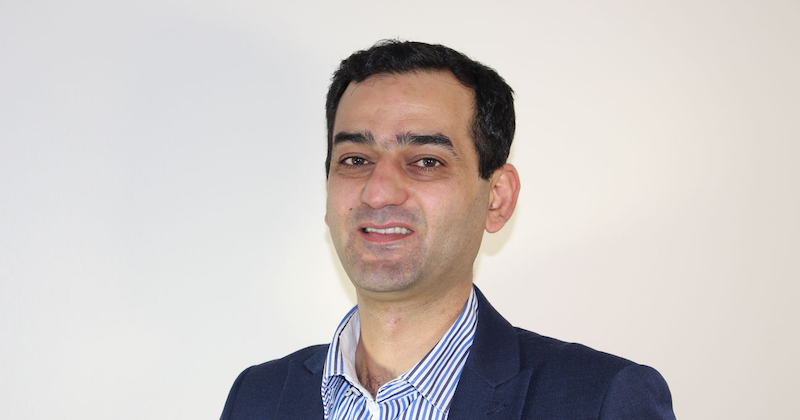
\includegraphics[width=1in,height=1.25in,clip,keepaspectratio]{a1.png}}]{Basel Magableh} 
Dr. Basel Magableh is  Lecturer in the School of Computer Science, Technological University Dublin. Basel has a BSc from the University of Yarmouk, Jordan, MSc from New York Institute of technology, USA and a PhD from Trinity College Dublin, Ireland. Basel has previously worked as a Chief Scientist in Mobile/Terminal Context Awareness in Huawei Technologies, Finland. He has also completed two post doctorate positions in UCD, and the Knowledge and Data Engineering Group (KDEG), Trinity College.
\end{IEEEbiography}

\begin{IEEEbiography}[{
\includegraphics[width=1in,height=1.25in,clip,keepaspectratio]{a3.png}}]{Muder Almani} 
Dr. Muder Almani is a Chair, Computer Information Systems Department / College of Information Technology Chair, Management Information Systems Department / College of Business Administration and Economics, Al-Hussein Bin Talal University, Ma'an - Jordan. Muder is actively researching in document handling, modems, peer-to-peer computing, power amplifiers, redundancy, security of data, storage management
\end{IEEEbiography}

\begin{IEEEbiography}[{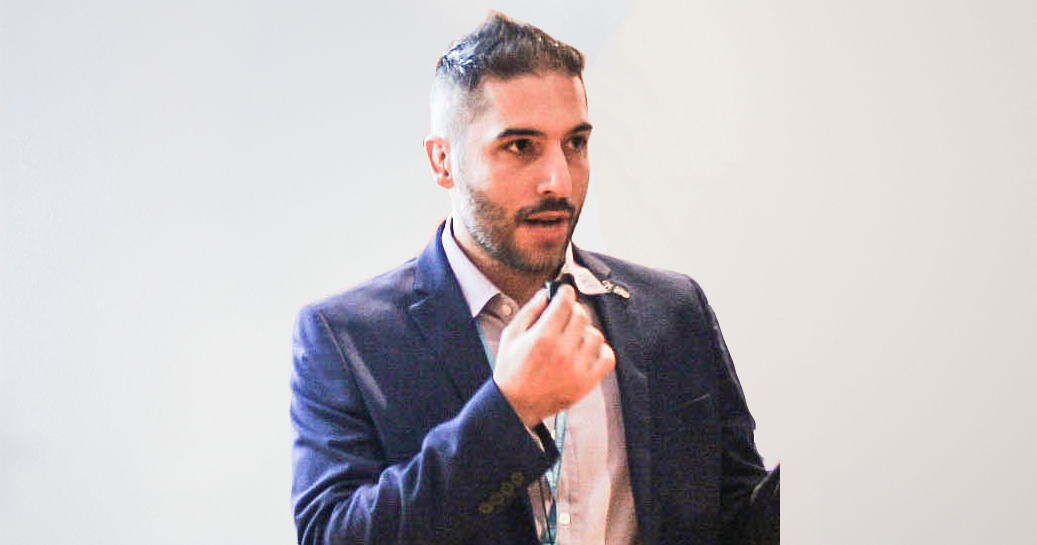
\includegraphics[width=1in,height=1.25in,clip,keepaspectratio]{DrLucaLongo380x200.png}}]{Luca Longo}  
Dr. Luca Longo is Lecturer in the School of Computer Science, Technological University Dublin.
Luca interests have always turned around Artificial Intelligence and innovative applications, especially applied to formal reasoning and the World Wide Web. Luca have completed a BSc with honours and a MSc awarded distinction both in Computer Science at the University of Insubria (Varese, Italy). Luca have obtained also a Postgraduate Diploma in statistics and a MSc in Health Informatics awarded distinction at Trinity College Dublin (Ireland). Luca successfully defended  PhD thesis in Artificial Intelligence at Trinity college Dublin. Additionally, Luca have recently obtained a Postgraduate diploma in Learning and Teaching at Dublin Institute of Technology, where Luca currently am tenured lecturer, covering both MSc and PhD courses.

Luca vision  is to formalise the ill-defined construct of human Mental Workload as a computational concept through deductive knowledge representation and reasoning techniques (Defeasible reasoning, Argumentation Theory) and inductive modelling techniques (Machine Learning). Field of applications includes Human-Computer Interaction, Education, NeuroScience, Universal Design.
\end{IEEEbiography}



 \EOD

\end{document}
